% answers.tex —— 1977 年·福建卷·文科 · 参考答案与详细解析片段
% 由 tools/generate_projects.py 依来源总账自 1977/1977_数学真题_福建文_试题.md + 1977/1977_数学真题_福建文_解析正文.md + 1977/1977_数学真题_福建文_答案要点.md 生成，勿手改（改源 MD 后重跑）


\begin{gktip}
固定源为 A3 单页题面，未附答案页。下文对可确定的小题给出独立推导；第 3(2)、第 4、第 5、第 6 的源面疑点保留在相应解析中。
\end{gktip}

\begin{answer}
\gksolhead{1}{}

\textbf{题目}：

\Needspace{5\baselineskip}
（1） 计算：

\nopagebreak[4]
\[
5-3\times\left[\left(-3\frac38\right)^{-\frac13}+1031\times\left(0.25-2^{-2}\right)\right]\div9^0
\]

（2） 求 $\cos(-840^\circ)$ 的值。

\Needspace{5\baselineskip}
（3） 化简：

\nopagebreak[4]
\[
\sqrt{(2x-3)^2}
\]

（4） 如图，在 $\triangle ABC$ 中，$MN\parallel BC$，$MN=1\ \mathrm{cm}$，$BC=3\ \mathrm{cm}$，$BM=AM+2$，求 $AM$ 的长。
\nopagebreak[4]
\begin{center}% 1977 年福建卷文科第 1(4) 题：三角形中的平行截线
\begin{tikzpicture}[scale=0.85]
  \coordinate (A) at (2.4,3.5);
  \coordinate (B) at (0,0);
  \coordinate (C) at (5.1,0);
  \coordinate (M) at ($(A)!0.42!(B)$);
  \coordinate (N) at ($(A)!0.42!(C)$);
  \draw[thick] (A)--(B)--(C)--cycle;
  \draw[thick] (M)--(N);
  \fill (A) circle (1.2pt) node[above] {$A$};
  \fill (B) circle (1.2pt) node[below left] {$B$};
  \fill (C) circle (1.2pt) node[below right] {$C$};
  \fill (M) circle (1.2pt) node[left] {$M$};
  \fill (N) circle (1.2pt) node[right] {$N$};
\end{tikzpicture}
\end{center}
\nopagebreak[4]
（5） 已知 $\lg3=0.4771$，$\lg x=3.4771$，求 $x$。

\Needspace{5\baselineskip}
（6） 求

\nopagebreak[4]
\[
\lim_{x\to1}\frac{x-1}{x^2-3x+2}
\]

（7） 求函数 $y=x^2+2x-4$ 的极小值。

（8） 已知 $\sin\alpha=\dfrac35$，$\dfrac\pi2<\alpha<\pi$，求 $\tan\alpha$ 的值。

\Needspace{5\baselineskip}
（9） 写出等比数列

\nopagebreak[4]
\[
-\frac29,\quad \frac2{27},\quad -\frac2{81},\quad\cdots
\]

的通项公式。

\Needspace{4\baselineskip}
\textbf{解析}

\gksubpart{（1）}

\Needspace{5\baselineskip}
因为 $-3\frac38=-\frac{27}{8}$，且

\nopagebreak[4]
\[
\left(-\frac{27}{8}\right)^{-\frac13}=-\frac23,
\qquad
0.25-2^{-2}=0,
\qquad 9^0=1
\]

\Needspace{5\baselineskip}
所以原式为

\nopagebreak[4]
\[
5-3\left(-\frac23+1031\times0\right)=7
\]

\gksubpart{（2）}

\nopagebreak[4]
\[
\cos(-840^\circ)=\cos840^\circ=\cos120^\circ=-\frac12
\]

\gksubpart{（3）}

\nopagebreak[4]
\[
\sqrt{(2x-3)^2}=\lvert2x-3\rvert
\]

\gksubpart{（4）}

\Needspace{5\baselineskip}
由 $MN\parallel BC$，有

\nopagebreak[4]
\[
\frac{AM}{AB}=\frac{MN}{BC}=\frac13
\]

\Needspace{5\baselineskip}
所以 $AB=3AM$，从而 $BM=AB-AM=2AM$。代入 $BM=AM+2$ 得

\nopagebreak[4]
\[
2AM=AM+2,
\qquad AM=2\ \mathrm{cm}
\]

\gksubpart{（5）}

\nopagebreak[4]
\[
\lg x=3.4771=3+0.4771=\lg1000+\lg3=\lg3000
\]

故 $x=3000$。

\gksubpart{（6）}

\Needspace{5\baselineskip}
因式分解分母并在 $x\ne1$ 时约去 $x-1$：

\nopagebreak[4]
\[
\lim_{x\to1}\frac{x-1}{x^2-3x+2}
=\lim_{x\to1}\frac1{x-2}=-1
\]

\gksubpart{（7）}

\Needspace{5\baselineskip}
配方得

\nopagebreak[4]
\[
y=x^2+2x-4=(x+1)^2-5
\]

所以极小值为 $-5$。

\gksubpart{（8）}

\Needspace{5\baselineskip}
因 $\alpha$ 是第二象限角，

\nopagebreak[4]
\[
\cos\alpha=-\sqrt{1-\sin^2\alpha}=-\frac45
\]

\Needspace{5\baselineskip}
故

\nopagebreak[4]
\[
\tan\alpha=\frac{\sin\alpha}{\cos\alpha}=-\frac34
\]

\gksubpart{（9）}

\Needspace{5\baselineskip}
相邻两项之比为

\nopagebreak[4]
\[
q=\frac{2/27}{-2/9}=-\frac13
\]

\Needspace{5\baselineskip}
首项为 $a_1=-2/9$，故通项为

\nopagebreak[4]
\[
a_n=-\frac29\left(-\frac13\right)^{n-1}
\]

\gkanswer{答案（1）：$7$。}

\gkanswer{答案（2）：$-\dfrac12$。}

\gkanswer{答案（3）：$\lvert2x-3\rvert$。}

\gkanswer{答案（4）：$AM=2\ \mathrm{cm}$。}

\gkanswer{答案（5）：$x=3000$。}

\gkanswer{答案（6）：$-1$。}

\gkanswer{答案（7）：极小值为 $-5$。}

\gkanswer{答案（8）：$-\dfrac34$。}

\gkanswer{答案（9）：$a_n=-\dfrac29\left(-\dfrac13\right)^{n-1}$。}

\end{answer}
\begin{answer}
\gksolhead{2}{}

\textbf{题目}：

\Needspace{5\baselineskip}
（1） 求函数

\nopagebreak[4]
\[
y=\frac{\lg(2-x)}{\sqrt{x-1}}
\]

的定义域。

\Needspace{5\baselineskip}
（2） 证明：

\nopagebreak[4]
\[
(\sin\alpha-\cos\alpha)^2+\sin2\alpha=1
\]

\Needspace{5\baselineskip}
（3） 解方程：

\nopagebreak[4]
\[
2\sqrt{x-3}+6=x
\]

\Needspace{5\baselineskip}
（4） 解不等式：

\nopagebreak[4]
\[
x^2-x-6<0
\]

\Needspace{5\baselineskip}
（5） 把分母有理化：

\nopagebreak[4]
\[
\sqrt{\frac{\sqrt5+\sqrt2}{\sqrt5-\sqrt2}}
\]

（6） 某中学革命师生自己动手油漆一个直径为 $1.2\ \mathrm m$ 的地球仪，如果每平方米面积需要油漆 $150$ 克，问共需油漆多少克？（答案保留整数。）

\Needspace{4\baselineskip}
\textbf{解析}

\gksubpart{（1）}

\Needspace{5\baselineskip}
对数真数要求 $2-x>0$，根式要求 $x-1\ge0$，分母还要求 $\sqrt{x-1}\ne0$，即 $x\ne1$。所以

\nopagebreak[4]
\[
x<2,\qquad x\ge1,\qquad x\ne1
\]

\Needspace{5\baselineskip}
定义域为

\nopagebreak[4]
\[
(1,2)
\]

\gksubpart{（2）}

\nopagebreak[4]
\[
\begin{aligned}
(\sin\alpha-\cos\alpha)^2+\sin2\alpha
&=\sin^2\alpha+\cos^2\alpha-2\sin\alpha\cos\alpha
+2\sin\alpha\cos\alpha\\
&=1
\end{aligned}
\]

\gksubpart{（3）}

\Needspace{5\baselineskip}
令 $t=\sqrt{x-3}\ge0$，则 $x=t^2+3$，方程化为

\nopagebreak[4]
\[
2t+6=t^2+3
\quad\Longleftrightarrow\quad
(t-3)(t+1)=0
\]

取 $t=3$，得 $x=12$。

\gksubpart{（4）}

\nopagebreak[4]
\[
x^2-x-6=(x-3)(x+2)<0
\]

故解集为 $-2<x<3$。

\gksubpart{（5）}

\nopagebreak[4]
\[
\begin{aligned}
\sqrt{\frac{\sqrt5+\sqrt2}{\sqrt5-\sqrt2}}
&=\sqrt{\frac{(\sqrt5+\sqrt2)^2}{5-2}}\\
&=\frac{\sqrt5+\sqrt2}{\sqrt3}
=\frac{\sqrt{15}+\sqrt6}{3}
\end{aligned}
\]

\gksubpart{（6）}

\Needspace{5\baselineskip}
地球仪视为球体，半径为 $0.6\ \mathrm m$，表面积为

\nopagebreak[4]
\[
4\pi r^2=4\pi(0.6)^2=1.44\pi\ \mathrm{m^2}
\]

\Needspace{5\baselineskip}
所需油漆质量为

\nopagebreak[4]
\[
150\times1.44\pi=216\pi\ \mathrm g
\approx678.24\ \mathrm g
\]

保留整数得 $678\ \mathrm g$（取 $\pi=3.14$）。

\gkanswer{答案（1）：$(1,2)$。}

\gkanswer{答案（2）：见解析版。}

\gkanswer{答案（3）：$x=12$。}

\gkanswer{答案（4）：$-2<x<3$。}

\gkanswer{答案（5）：$\dfrac{\sqrt{15}+\sqrt6}{3}$。}

\gkanswer{答案（6）：$216\pi\ \mathrm g\approx678\ \mathrm g$（取 $\pi=3.14$）。}

\end{answer}
\begin{answer}
\gksolhead{3}{}

\textbf{题目}：

某农机厂开展“工业学大庆”运动，在十月份生产拖拉机 $1000$ 台。这样，一月至十月的产量恰好完成全年生产任务。工人同志为了加速农业机械化，计划在年底前再生产 $2310$ 台。

（1） 求十一月、十二月份每月增长率；

（2） 原计划年产拖拉机多少台？

\Needspace{4\baselineskip}
\textbf{解析}

\gksubpart{（1）}

\Needspace{5\baselineskip}
若按题意把十一月、十二月理解为从十月的 $1000$ 台按同一月增长率递增，设增长因子为 $q=1+r$，则

\nopagebreak[4]
\[
1000q+1000q^2=2310
\quad\Longleftrightarrow\quad
q^2+q-2.31=0
\]

\Needspace{5\baselineskip}
解得 $q=1.1$ 或 $q=-2.1$。增长因子取正，故

\nopagebreak[4]
\[
r=0.1=10\%
\]

这是在该隐含递增假设下的候选解；源题面未把这一假设明确写出。

\gksubpart{（2）}

源题面只说明“一月至十月的产量恰好完成全年生产任务”，但没有给出一月至十月各月产量，也没有给出其变化规律。因此原计划年产量就是一月至十月产量之和，但不能由当前固定源唯一计算出数值。

\gkanswer{答案（1）：按十月产量 $1000$ 台、十一月至十二月按相同月增长率递增的条件，可得每月增长率 $10\%$。}

\gkanswer{答案（2）：源题面未给出一月至十月各月产量或其变化规律，无法由当前信息唯一确定原计划年产量，待补充条件或权威版本。}

\end{answer}
\begin{answer}
\gksolhead{4}{}

\textbf{题目}：

求抛物线 $y^2=9x$ 和圆 $x^2+y^2=36$ 在第一象限的交点处的切线方程。

\Needspace{4\baselineskip}
\textbf{解析}

\Needspace{5\baselineskip}
联立抛物线和圆：

\nopagebreak[4]
\[
y^2=9x,\qquad x^2+y^2=36
\]

\Needspace{5\baselineskip}
得到 $x^2+9x-36=0$。第一象限取 $x=3$，于是 $y=3\sqrt3$，交点为

\nopagebreak[4]
\[
A=(3,3\sqrt3)
\]

\Needspace{5\baselineskip}
抛物线求导得 $2yy'=9$，所以在 $A$ 点的斜率为 $\sqrt3/2$，切线为

\nopagebreak[4]
\[
y-3\sqrt3=\frac{\sqrt3}{2}(x-3)
\]

\Needspace{5\baselineskip}
圆求导得 $2x+2yy'=0$，所以在 $A$ 点的斜率为 $-1/\sqrt3$，切线为

\nopagebreak[4]
\[
x+\sqrt3y-12=0
\]

两条切线不同；源题面使用单数“切线方程”，故不能在没有补充说明时选定其中一条。

\gkanswer{答案：第一象限交点为 $(3,3\sqrt3)$；抛物线切线为 $y-3\sqrt3=\dfrac{\sqrt3}{2}(x-3)$，圆切线为 $x+\sqrt3y-12=0$。源题面使用单数“切线方程”，未说明求哪一条，待核。}

\end{answer}
\begin{answer}
\gksolhead{5}{}

\textbf{题目}：

\Needspace{5\baselineskip}
已知双曲线

\nopagebreak[4]
\[
\frac{x^2}{24\alpha}-\frac{y^2}{16\cot\alpha}=1\quad(\alpha\text{ \text{为锐角}})
\]

和圆 $(x-m)^2+y^2=r^2$ 相切于点 $A(4\sqrt3,4)$，求 $\alpha\text{、}m\text{、}r$ 的值。

\Needspace{4\baselineskip}
\textbf{解析}

\Needspace{5\baselineskip}
将 $A=(4\sqrt3,4)$ 代入源面双曲线，得到

\nopagebreak[4]
\[
\frac{48}{24\alpha}-\frac{16}{16\cot\alpha}=1
\quad\Longleftrightarrow\quad
\frac2\alpha-\tan\alpha=1
\]

其中三角函数的角度单位与分母中的 $\alpha$ 的数值单位未由源面说明。若把 $\alpha$ 按弧度数处理，锐角方程的数值根约为 $\alpha=0.8924934\ \mathrm{rad}=51.1361^\circ$。

\Needspace{5\baselineskip}
双曲线在 $A$ 点的切线斜率为

\nopagebreak[4]
\[
k_h=\frac{2x\cot\alpha}{3\alpha y}
=\frac{2\sqrt3\cot\alpha}{3\alpha}
\]

\Needspace{5\baselineskip}
圆心为 $(m,0)$ 的圆在 $A$ 点切线斜率为 $-(4\sqrt3-m)/4$，故

\nopagebreak[4]
\[
m=4\sqrt3+\frac{8\sqrt3\cot\alpha}{3\alpha},
\qquad
r=\sqrt{(4\sqrt3-m)^2+16}
\]

按上述弧度候选根数值计算，得到 $m\approx11.0987$、$r\approx5.7786$。由于源式参数形式异常且无答案页，这些数值只能作为按字面解释的候选，不能当作已核定标准答案。

\gkanswer{答案：按源式可列 $\dfrac2\alpha-\tan\alpha=1$；若取其锐角数值根，则 $\alpha\approx51.1361^\circ$，$m\approx11.0987$，$r\approx5.7786$。由于源式含 $24\alpha$ 且无答案页，暂作按字面计算的候选值，待权威版本核对。}

\end{answer}
\begin{answer}
\gksolhead{6}{}

\textbf{题目}：

某大队在农田基本建设的规划中，要测定被障碍物隔开的两点 $A\text{、}P$ 之间的距离。他们土法上马，在障碍物的两侧选取两点 $B$ 和 $C$（如图），测得 $AB=AC=50\ \mathrm m$，$\angle BAC=60^\circ$，$\angle ABP=120^\circ$，$\angle ACP=135^\circ$，求 $A$ 和 $P$ 之间的距离。（答案可用最简根式表示。）
\nopagebreak[4]
\begin{center}% 1977 年福建卷文科第 6 题：障碍物两侧测距示意图
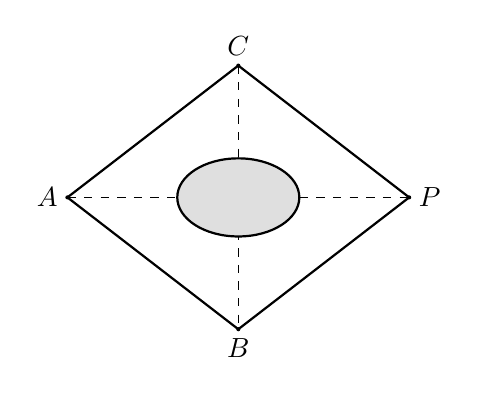
\begin{tikzpicture}[scale=0.62]
  \coordinate (A) at (0,0);
  \coordinate (P) at (7.0,0);
  \coordinate (C) at (3.5,2.7);
  \coordinate (B) at (3.5,-2.7);
  \draw[thick] (A)--(C)--(P)--(B)--cycle;
  \draw[dashed] (A)--(P);
  \draw[dashed] (C)--(B);
  \fill[gray!25] (3.5,0) ellipse (1.25 and 0.8);
  \draw[thick] (3.5,0) ellipse (1.25 and 0.8);
  \fill (A) circle (1.2pt) node[left] {$A$};
  \fill (P) circle (1.2pt) node[right] {$P$};
  \fill (C) circle (1.2pt) node[above] {$C$};
  \fill (B) circle (1.2pt) node[below] {$B$};
\end{tikzpicture}
\end{center}
\nopagebreak[4]
\Needspace{4\baselineskip}
\textbf{解析}

由 $AB=AC=50$ 且 $\angle BAC=60^\circ$，可知 $\triangle ABC$ 为等边三角形。取 $A=(0,0)$、$B=(25,-25\sqrt3)$、$C=(25,25\sqrt3)$，则从 $B$ 出发与 $BA$ 成普通角 $120^\circ$ 的射线方向只能为 $0^\circ$ 或 $240^\circ$；从 $C$ 出发与 $CA$ 成普通角 $135^\circ$ 的射线方向只能为 $15^\circ$ 或 $105^\circ$。

前一组射线的纵坐标不大于 $-25\sqrt3$，后一组射线的纵坐标不小于 $25\sqrt3$，四种组合均不能相交于题图所示的同一点 $P$。因此当前固定源的角度条件在普通平面角解释下不相容，不能可靠给出 $AP$ 的唯一长度；需要更清晰源卷或权威勘误确认。

\gkanswer{答案：按普通平面角定义，$AB=AC$ 且 $\angle BAC=60^\circ$ 使 $\triangle ABC$ 为等边三角形；此时从 $B$、$C$ 按题给 $120^\circ$、$135^\circ$ 作射线不能得到图示同一交点 $P$，当前源面条件不相容，无法给出可靠唯一距离，待核。}

\end{answer}